\section{Własne funkcje krzyżowania i mutacji}

\subsection{Krzyżowanie}

\subsubsection{Funkcja testowa}
Testu algorytmu zostały wykonane dla funkcji wielomodalnej nr. 13 z biblioteki \textit{cec2013}.

\begin{figure}[H]
	\centering
	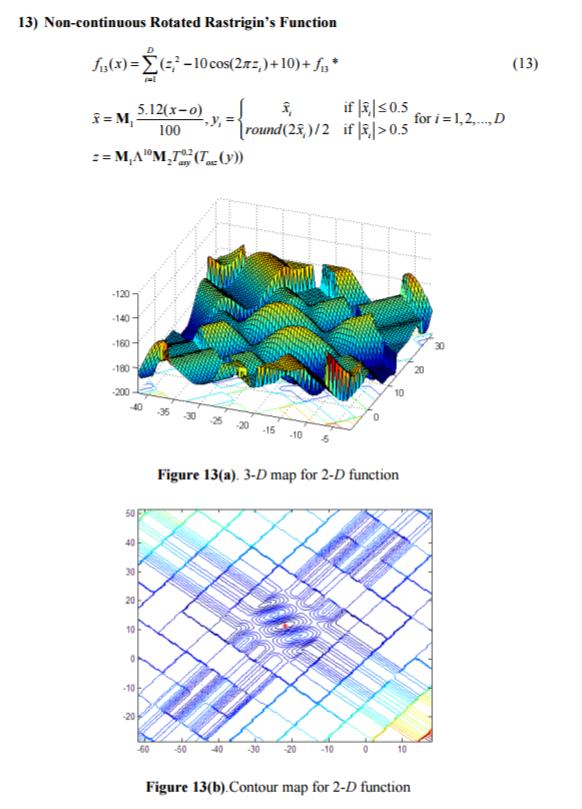
\includegraphics[scale=0.9]{f13}
	\caption{Funkcja testowa}
\end{figure}

\subsubsection{Założenia testów}

W celu przetestowania możliwości użycia własnej funkcji krzyżowania zmodyfikowana została standardowa funkcja \textit{gareal\_waCrossover} z pakietu \textit{GA}.
Oryginalny współczynnik służący do określenia proporcji parametrów rodziców w potomstwie,
określony przez rozkład jednostajny na zakresie (0-1) zastąpiony został wartością stałą, wynoszącą odpowiednio 0,6 i 0,4 dla rodziców.

Wykonane zostały badania przy różnych wartościach parametru odpowiadającego za szansę krzyżowania oraz wielkości populacji.
Do analizy wyników posłużyły wartość znalezionego minimum oraz liczba iteracji, po których algorytm kończył działanie.
Pozwala to analizować jednocześnie jakość wyniku i czas potrzebny na jego znalezienie - co w przypadku rzeczywistych zastosowań ma równie duże znaczenie.

Wszystkie przedstawione wyniki są uśrednieniem wyników z 30 uruchomień algorytmu, maksymalna ilość iteracji to 250, obszar poszukiwań minimum:

\begin{equation}
x\in [-60, 10]
\nonumber
\end{equation}
\begin{equation}
y\in [-50, 20]
\nonumber
\end{equation}

Pozostałe parametry przyjmowały wartości domyślne dla pakietu \textit{GA}.
\subsubsection{Wyniki w zależności od prawdopodobieństwa krzyżowania}
\begin{figure}[H]
	\centering
	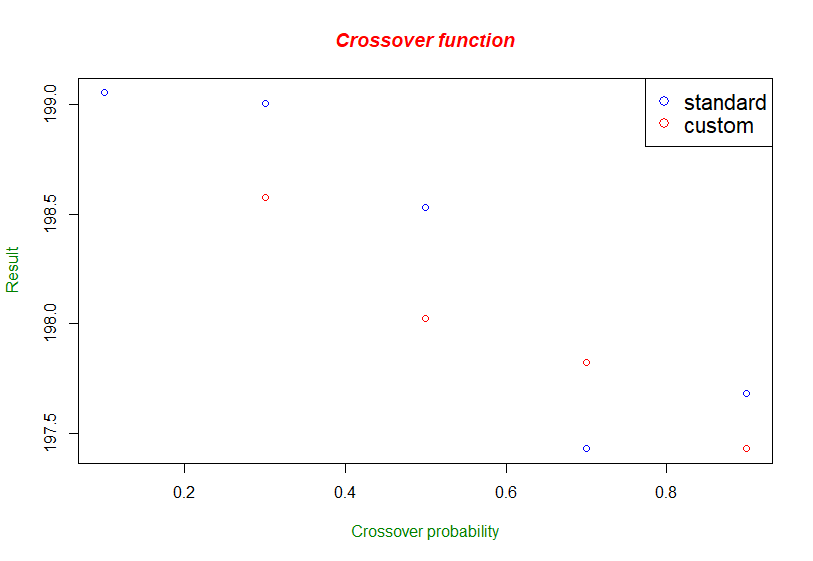
\includegraphics[scale=0.5]{custCrossover_pcross_result}
	\caption{Rezultat optymalizacji dla różnych wartości prawdopodobieństwa krzyżowania}

\end{figure}

\begin{figure}[H]
	\centering
	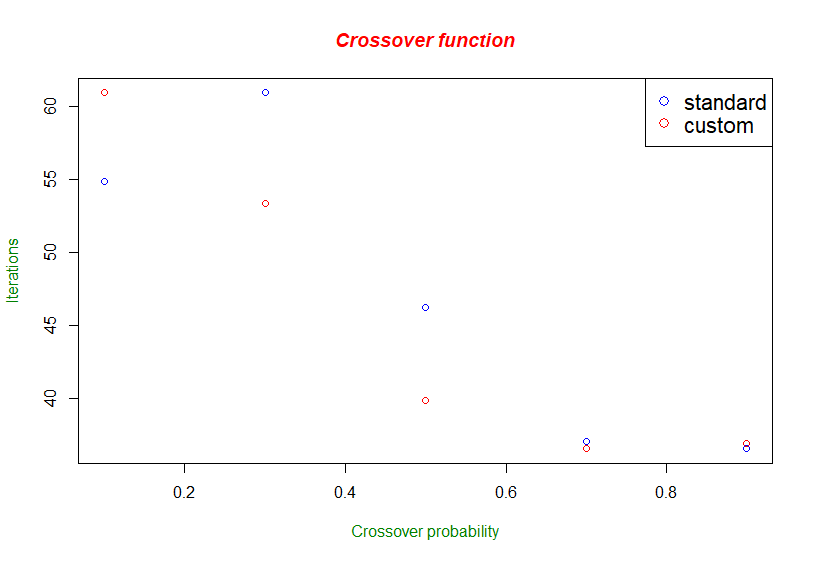
\includegraphics[scale=0.5]{custCrossover_pcross_iterations}
	\caption{Ilość iteracji dla różnych wartości prawdopodobieństwa krzyżowania}
\end{figure}


\subsubsection{Wyniki w zależności od wielkości populacji}

\begin{figure}[H]
	\centering
	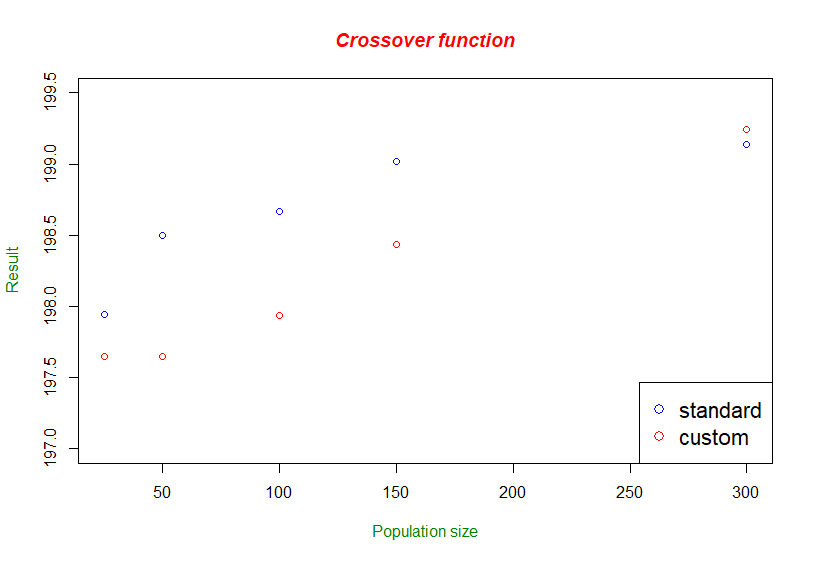
\includegraphics[scale=0.5]{custCrossover_popSize_results}
	\caption{Rezultat optymalizacji dla różnych wielkości populacji}

\end{figure}

\begin{figure}[H]
	\centering
	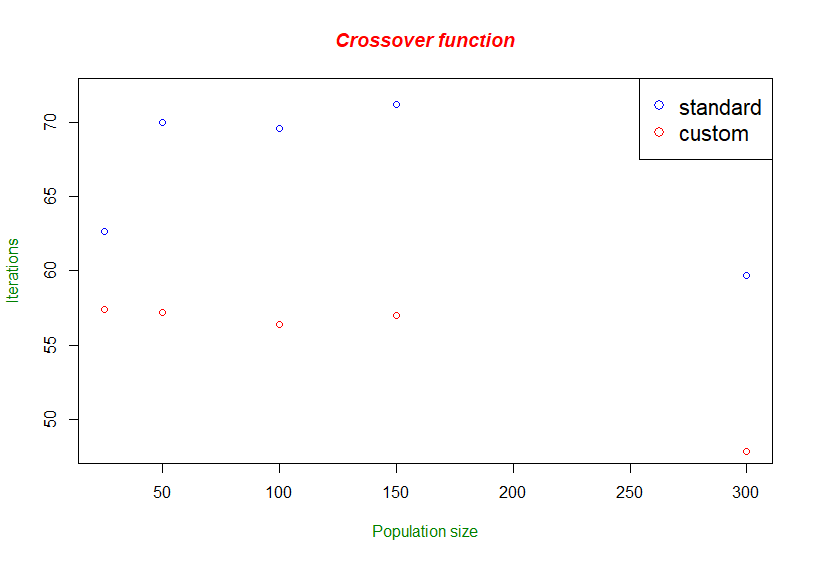
\includegraphics[scale=0.5]{custCrossover_popSize_iterations}
	\caption{Ilość iteracji dla różnych wielkości populacji}
\end{figure}

\subsubsection{Wnioski}

Modyfikacja algorytmu poprzez wyeliminowanie zmiennej losowej z funkcji krzyżowania spowodowała pogorszenie osiąganych przez algorytm genetyczny wyników.
Algorytm genetyczny po modyfikacji krzyżowania słabiej odnajduje minimum w ramach pojedynczego minimum lokalnego co przedstawia się w
mniejszej ilości iteracji wykonywanych przez algorytm - przy braku postępu funkcja stopu kończy działanie programu.

\newpage

\subsection{Mutacja}

\subsubsection{Funkcja testowa}

Testy zostały przeprowadzone dla tej samej funkcji wielomodalnej, co w przypadku testów podmiany funkcji krzyżowania, czyli funkcji 13 z pakietu
cec2013.

\subsubsection{Założenia testów}

W ramach testów zachowania się GA przy zmianie funkcji mutacji, posłużono się zmodyfikowaną funkcją \textit{gareal\_nraMutation (non uniform random mutation)}
z pakietu \textit{GA}.

W funkcji zmieniono współczynnik tłumienia (\textit{dempening factor}) z obliczanego na postawie bieżącej iteracji oraz maksymalnej liczby iteracji na
stały o wartości 0.1.

Badania wykonano zmieniając wartości szansy mutacji oraz wielkości populacji.
Reszta parametrów, jest taka sama, jak w przypadku podmiany funkcji krzyżowania:

\begin{itemize}
\item analizę wniosków oparto o wartość znalezionego minimum i liczbę iteracji, po których algorytm kończył działanie
\item wyniki są uśrednieniem 30 uruchomień algorytmu
\item maksymalna ilość iteracji to 250
\item obszar poszukiwania minimum:

\begin{equation}
x\in [-60, 10]
\nonumber
\end{equation}
\begin{equation}
y\in [-50, 20]
\nonumber
\end{equation}

\end{itemize}


\subsubsection{Wyniki w zależności od prawdopodobieństwa mutacji}

\begin{figure}[H]
	\centering
	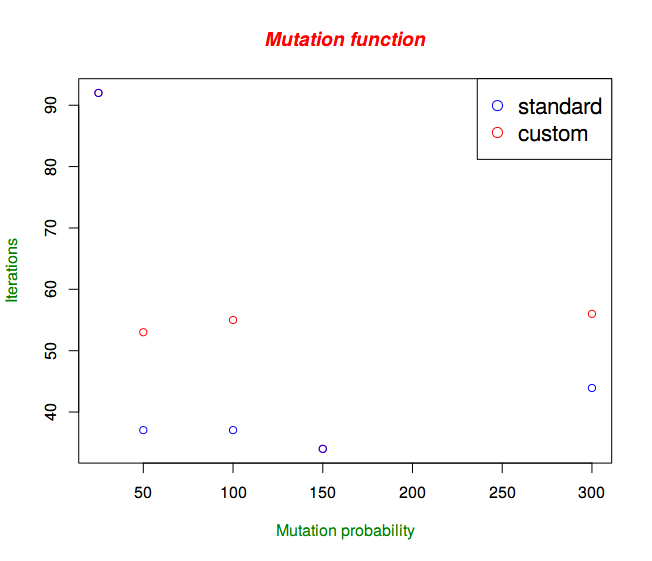
\includegraphics[scale=0.5]{custMutation_pmut_iteration}
	\caption{Ilość iteracji dla różnych wartości prawdopodobieństwa mutacji}
\end{figure}

\begin{figure}[H]
	\centering
	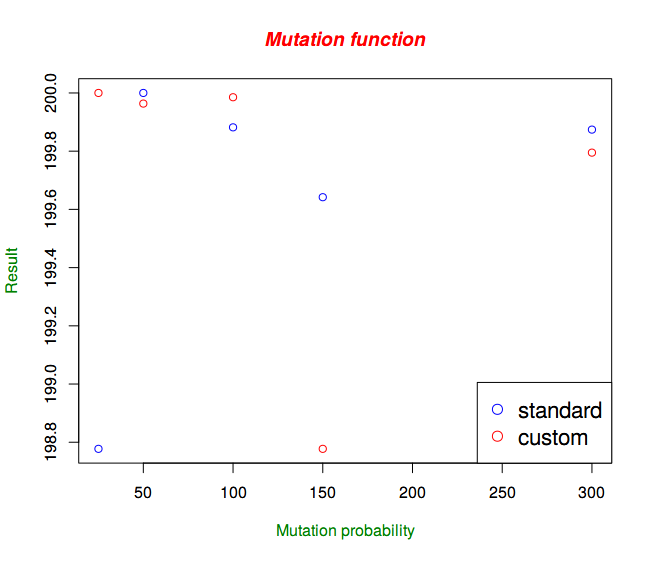
\includegraphics[scale=0.5]{custMutation_pmut_result}
	\caption{Rezultat optymalizacji dla różnych wartości prawdopodobieństwa mutacji}
\end{figure}

\subsubsection{Wyniki w zależności od rozmiaru populacji}

\begin{figure}[H]
	\centering
	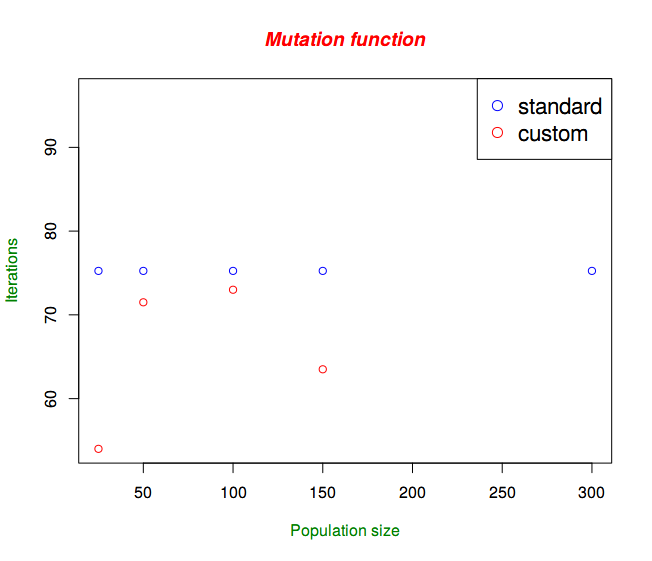
\includegraphics[scale=0.5]{custMutation_popSize_iteration}
	\caption{Ilość iteracji  dla różnych rozmiarów populacji}
\end{figure}

\begin{figure}[H]
	\centering
	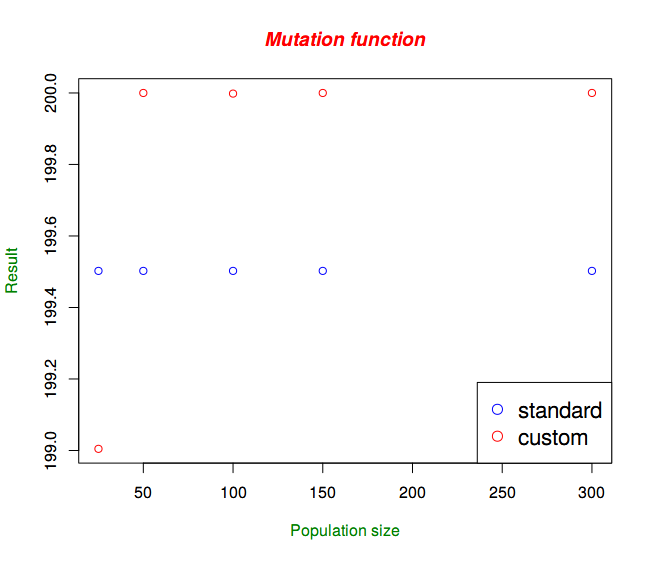
\includegraphics[scale=0.5]{custMutation_popSize_result}
	\caption{Rezultat optymalizacji  dla różnych rozmiarów populacji}
\end{figure}

\subsubsection{Wnioski}

Modyfikacja algorytmu ponownie spowodowała znaczące pogorszenie osiąganych przez algorytm genetyczny wyników.

Algorytm genetyczny po modyfikacji mutacji nieco lepiej za to odnajduje minimum w ramach pojedynczego minimum lokalnego - ga wykonuje więcej iteracji
przed sytuacją, w której postęp nie występuje.
Sytuacja ta ma miejsce kiedy modyfikowane jest prawdopodobieństwo mutacji.

